%------------------------------------------
%	$Id$
%
%	The GMT Documentation Project
%	Copyright (c) 2000-2011.
%	P. Wessel, W. H. F. Smith, R. Scharroo, and J. Luis
%------------------------------------------
%
\chapter{Chart of octal codes for characters}
\label{app:F}
\thispagestyle{headings}
\index{Characters!octal}
\index{Octal characters}
\index{Font!standard}
\index{Font!ISOLatin1}

The characters and their octal codes in the Standard and ISOLatin1 encoded fonts
are shown in Figure~\ref{fig:GMT_App_F_text}.  Light red areas signify codes reserved for
control characters.  In order to use all the extended characters (shown in the light green boxes) you need to
set \textbf{PS\_CHAR\_ENCODING} to Standard+ or ISOLatin1+ in your \filename{gmt.conf} file\footnote{If you chose
SI units during the installation then the default encoding is ISOLatin1+, otherwise it is Standard+.}.

\begin{figure}[h]
   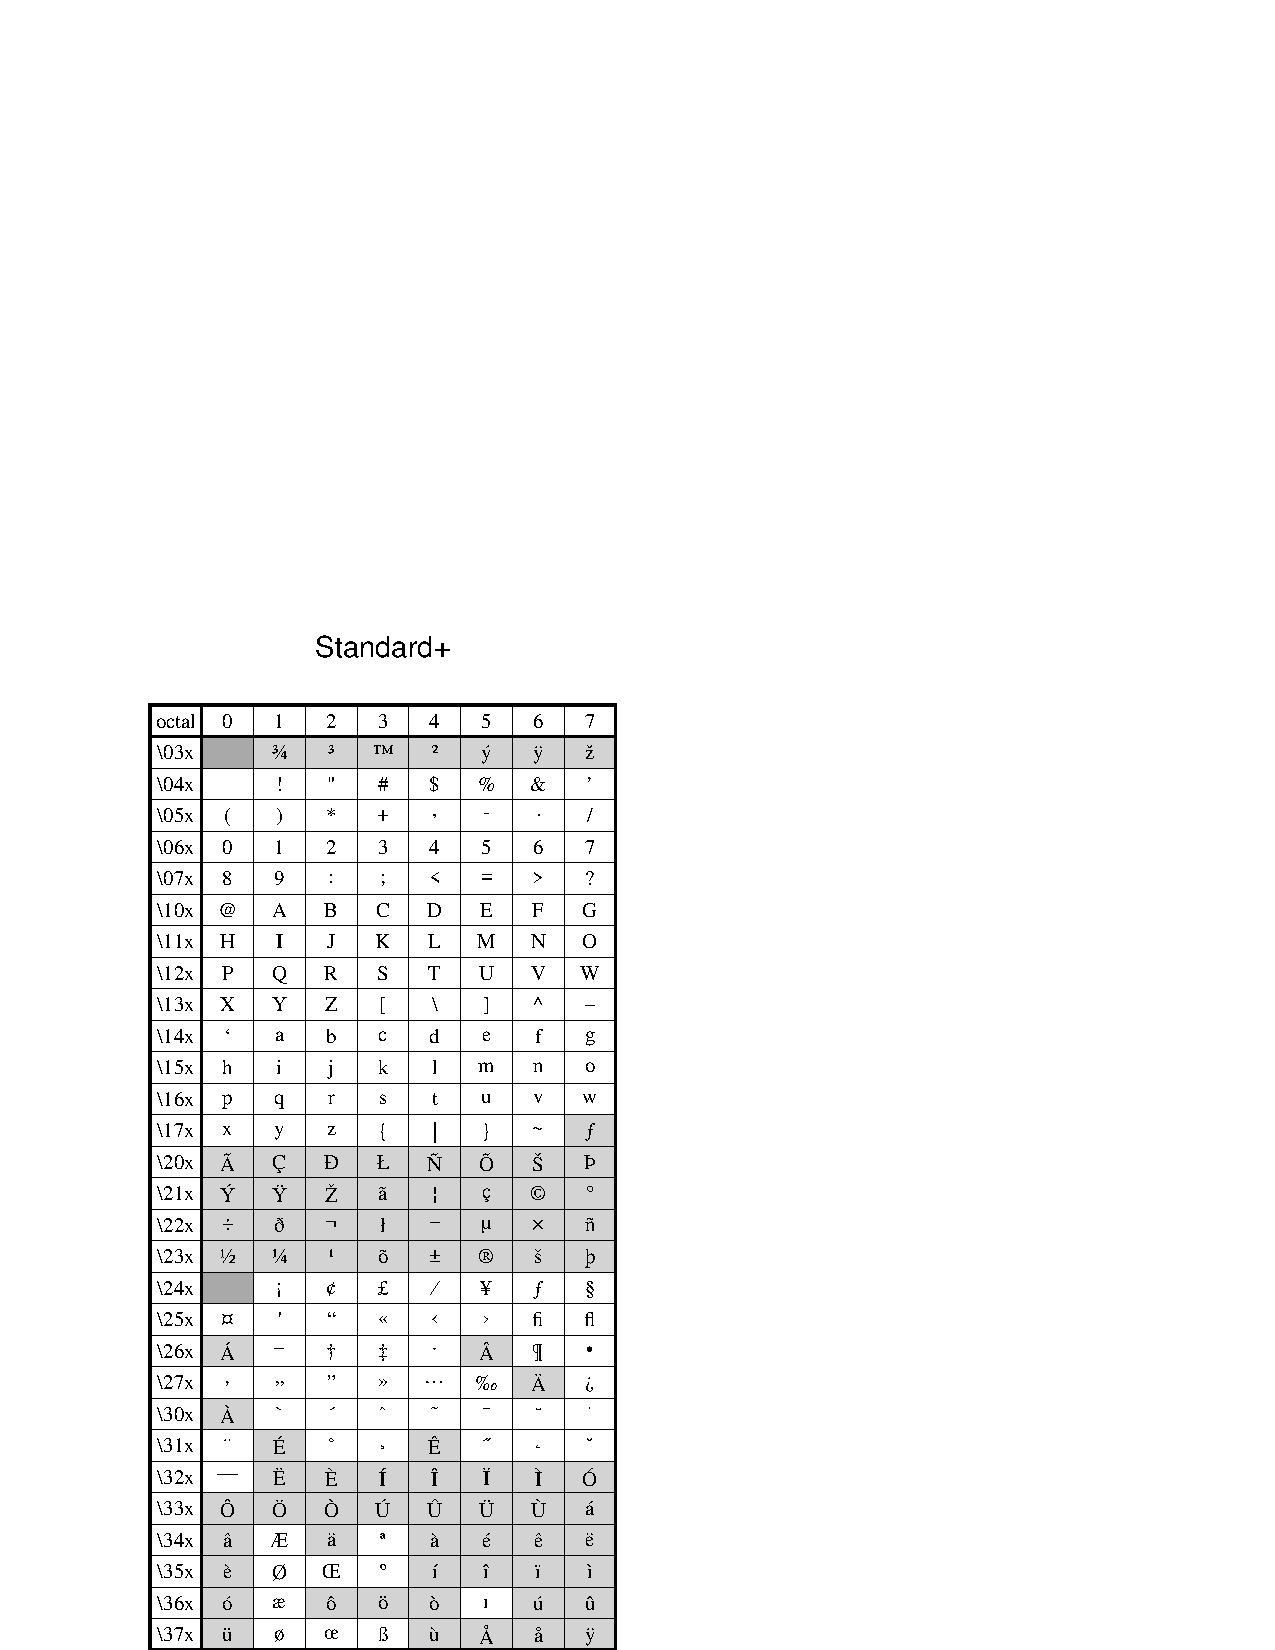
\includegraphics[scale=0.92]{GMT_App_F_stand+}\hfill
   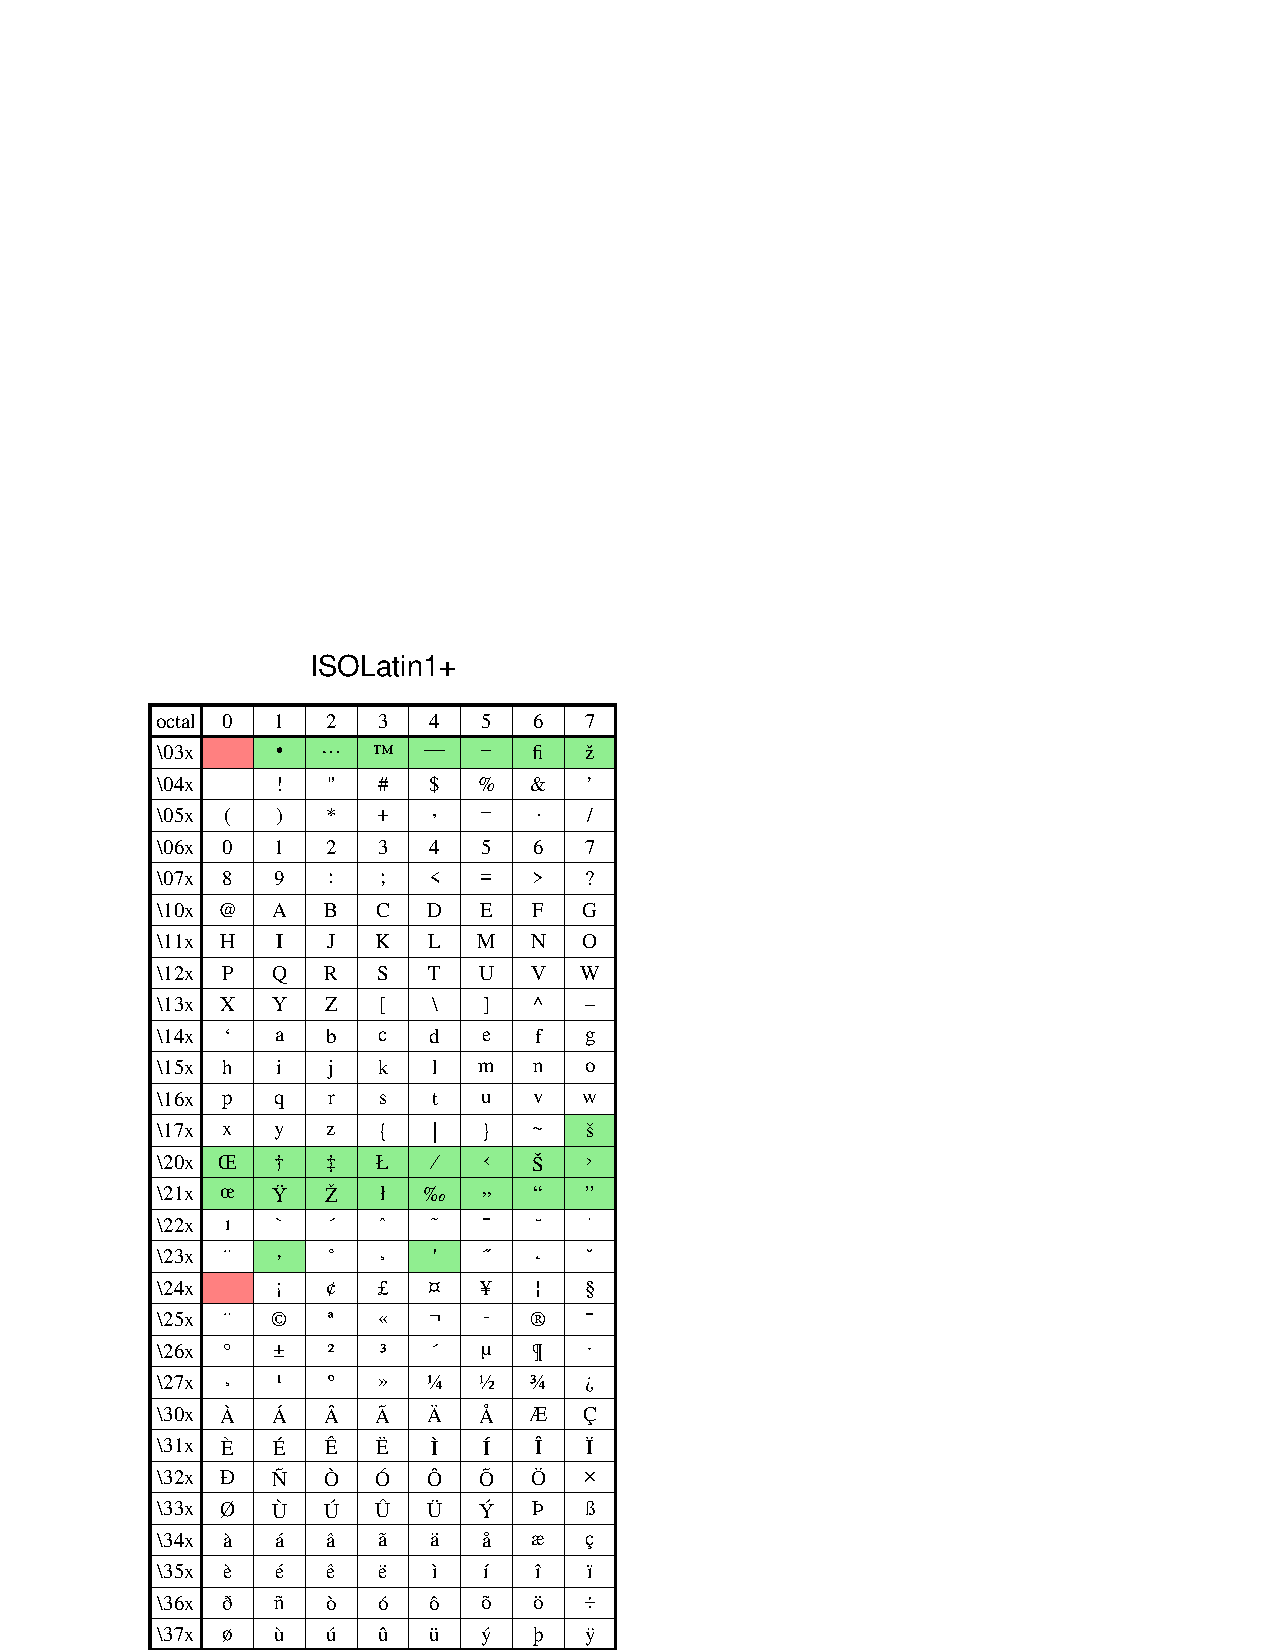
\includegraphics[scale=0.92]{GMT_App_F_iso+}
   \caption{Octal codes and corresponding symbols for StandardEncoding (left)
   and ISOLatin1Encoding (right) fonts.}
   \label{fig:GMT_App_F_text}
\end{figure}

\clearpage

\index{Symbol font}
\index{Font!symbol}
\index{Font!ZapfDingbats}

The chart for the Symbol character set (\GMT\ font number 12) and Pifont ZapfDingbats character set
(font number 34)
are presented in Figure~\ref{fig:GMT_App_F_symbol} below. The octal code is obtained by appending the
column value to the $\backslash$?? value, e.g., $\partial$ is
$\backslash$266 in the Symbol font.  The euro currency symbol is $\backslash$240 in the Symbol font and will
print if your printer supports it (older printer's firmware will not know about the euro).

\begin{figure}[h]
   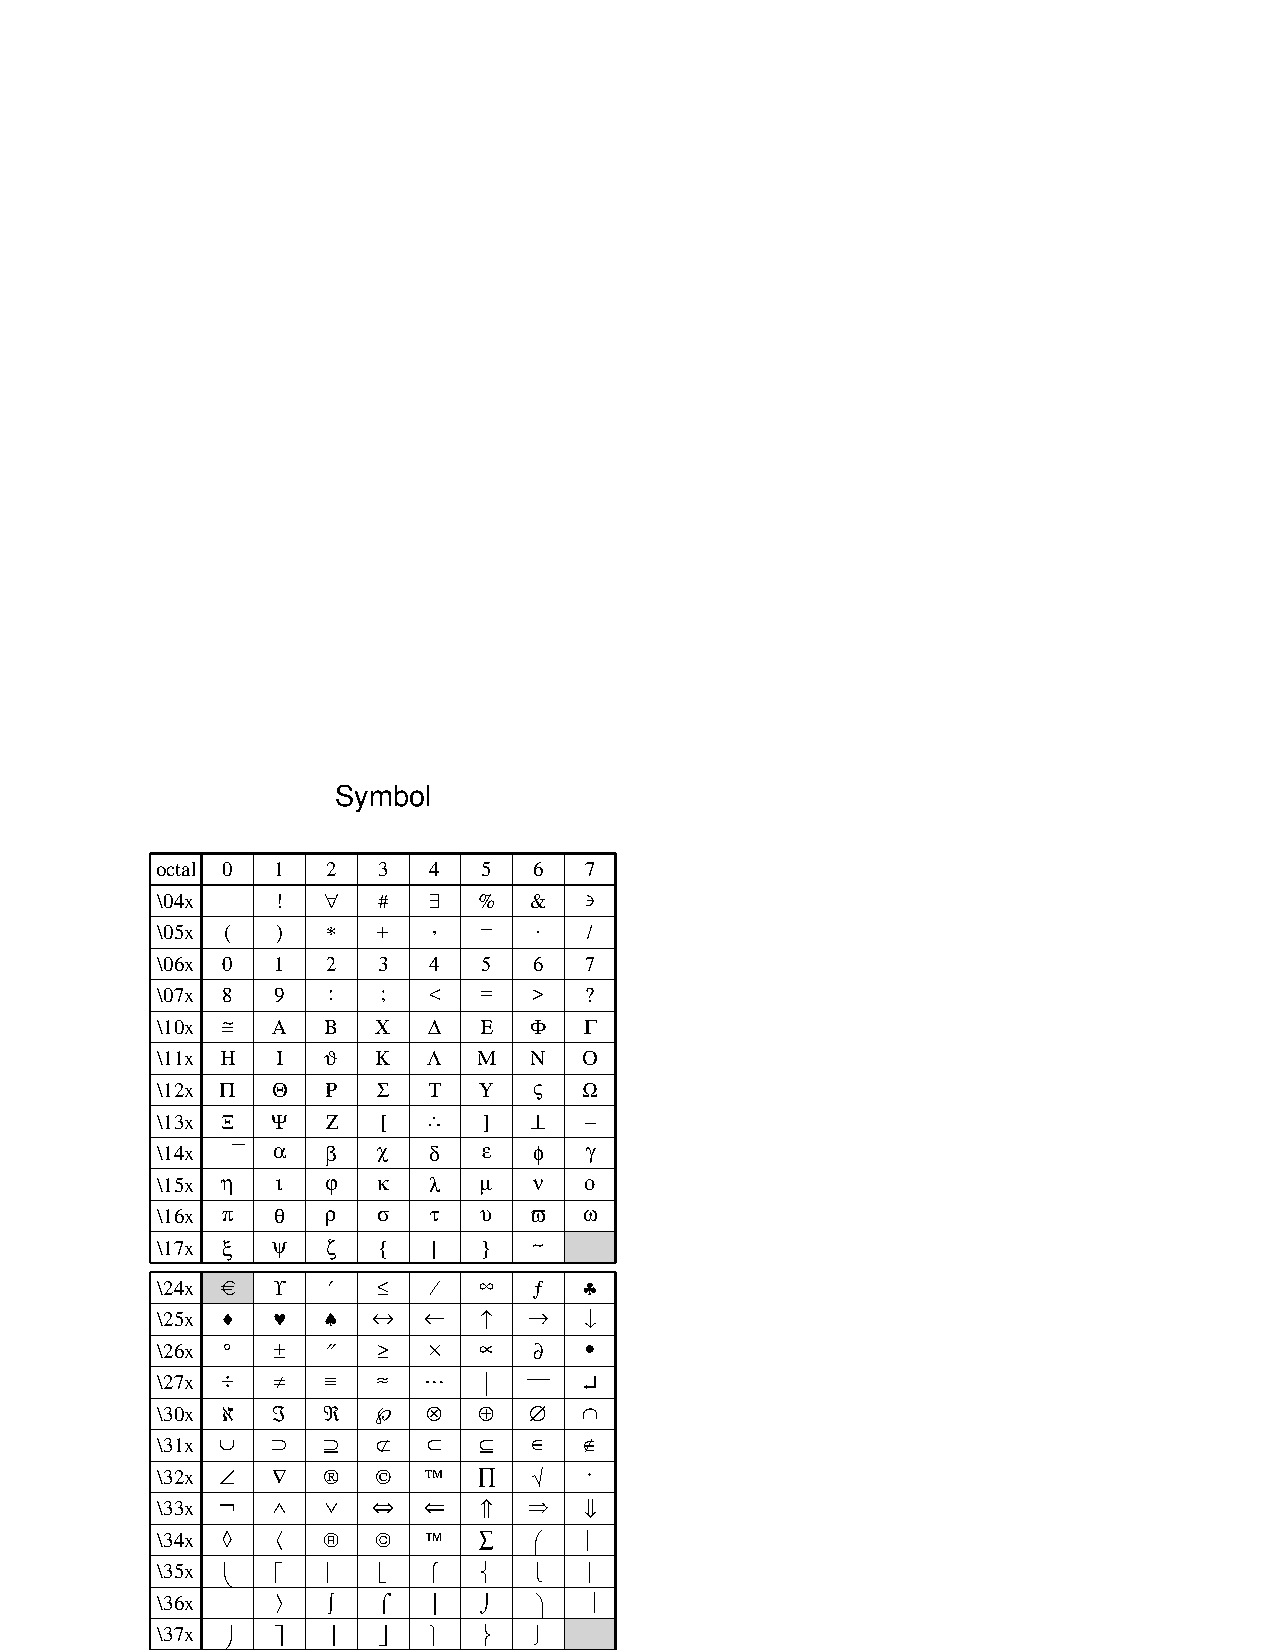
\includegraphics[scale=0.92]{GMT_App_F_symbol}\hfill
   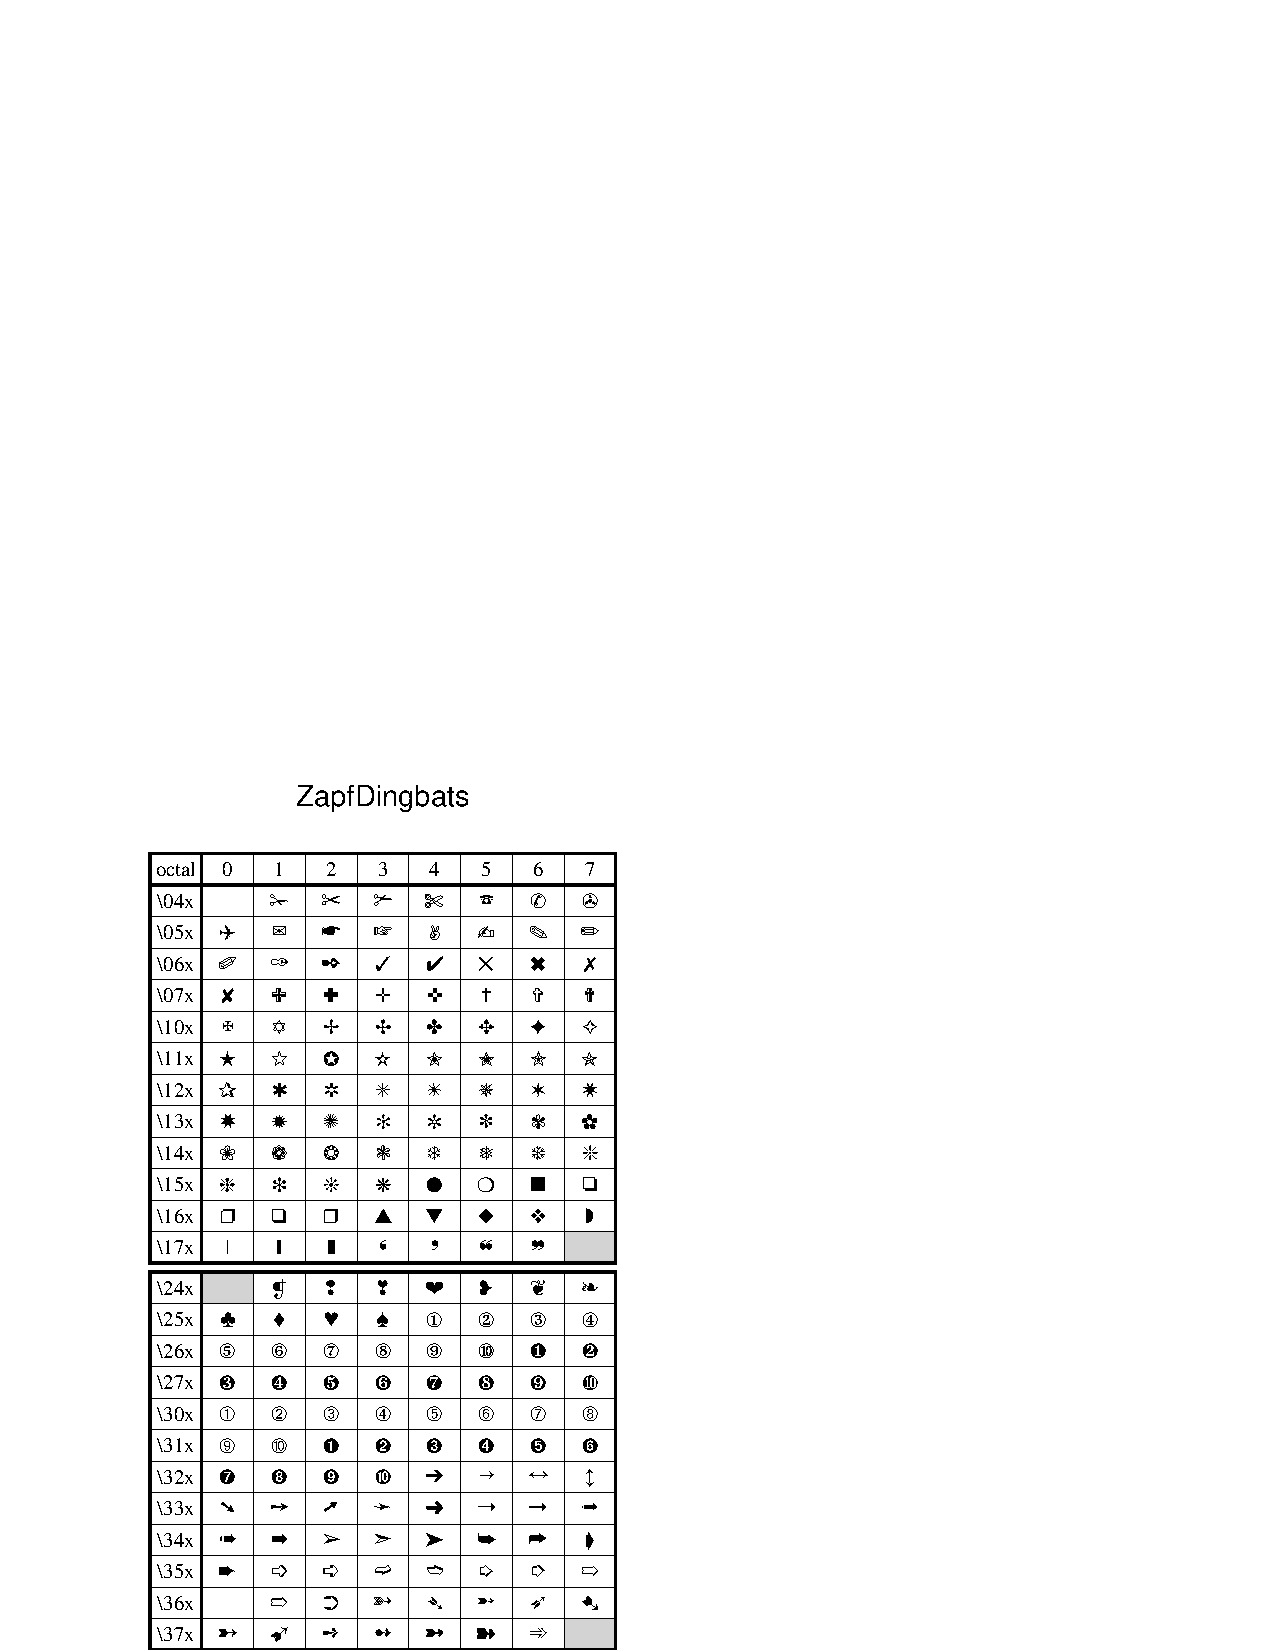
\includegraphics[scale=0.92]{GMT_App_F_dingbats}
   \caption{Octal codes and corresponding symbols for Symbol (left)
   and ZapfDingbats (right) fonts.}
   \label{fig:GMT_App_F_symbol}
\end{figure}
